\documentclass[12pt,a4paper,oneside]{article}
\usepackage{graphicx}
\usepackage{float} %for [H]


\usepackage{titlepic}
\usepackage[utf8]{inputenc}
\usepackage[left=1.1in,right=1.1in, top=1in, bottom= 1in]{geometry}
\usepackage[none]{hyphenat} % Avoids to go out of margin
\usepackage{subfiles}

% Font size of figure smaller than normal size:
\usepackage{caption}
\captionsetup[figure]{font=small}
\linespread{1.2}

% --------------------------------------------- %

\title{Homework 2}	                                    % Title
\author{Flavio Maiorana 2051396}				        % Authors separated by \\
\date{\today}								            % Date

\makeatletter
\let\thetitle\@title
\let\theauthor\@author
\let\thedate\@date
\makeatother

\begin{document}

\begin{titlepage}
	\centering
    \vspace*{0.5 cm}
    
\includegraphics[scale = 0.75]{figures/SapienzaLogo.pdf}\\[1.0 cm]	% University Logo

    % \vspace*{-0.4cm}
    % \textsc{\large DIAG}\\[2.0 cm]	% Department Name
    % \vspace*{1cm}

    { \fontsize{20.74pt}{18.5pt}\selectfont\bfseries \thetitle \par } % Title

    \vspace*{0.25cm}
    \textsc{\Large Machine Learning}\\[0.5 cm] % Course Name

    \vspace*{2.6cm}
	% \begin{minipage}{0.4\textwidth} % 0.4
	% 	\begin{flushleft} \large
	% 		\textbf{Professors:}\\
	% 		Professor Name\\
	% 	\end{flushleft}
	% \end{minipage}~
	\begin{minipage}{0.3\textwidth} %0.4
		\begin{flushright} \large
		\begin{minipage}{1\textwidth}
		\begin{flushleft} \large
			\textbf{Students:} \\
			\theauthor
        \end{flushleft}
        \end{minipage}
		\end{flushright}
	\end{minipage}\\[3.85 cm]

    \vspace{2cm}
    \rule{\linewidth}{0.2 mm} \\[0.3 cm]
    \vspace*{-0.2cm}
    Academic Year 2023/2024
\end{titlepage}
\newpage


\section{Data visualization and preprocessing}

First of all, it could be useful to gain some insight one how the dataaset is
made. The available data is already split into training and testing set. We
will consider the test split only in the evaluation phase (to prevent
data leakage).

\begin{verbatim}[Dataset for Training]
    N Examples: 6369
    N Classes: 5
    Classes: [0 1 2 3 4]
    - Class 0: 1000 (15.701051970482022)
    - Class 1: 1500 (23.551577955723033)
    - Class 2: 1500 (23.551577955723033)
    - Class 3: 2000 (31.402103940964043)
    - Class 4: 369 (5.7936881771078665)
\end{verbatim}

Some comments: the dataset is highly imbalanced. There are 

\newpage

\subsection{Preprocessing for evaluation}



\section{Model}

Different approaches can be used to solve this problem. We will treat mainly 4
models: KNN, SVM (linear and nonlinear), Gaussian Naive Bayes and Softmax
Regression. They will be compared based on the same train-test split.

\subsection{KNN}

\begin{verbatim} [Dataset 1]
\end{verbatim}

\begin{figure}[H]
    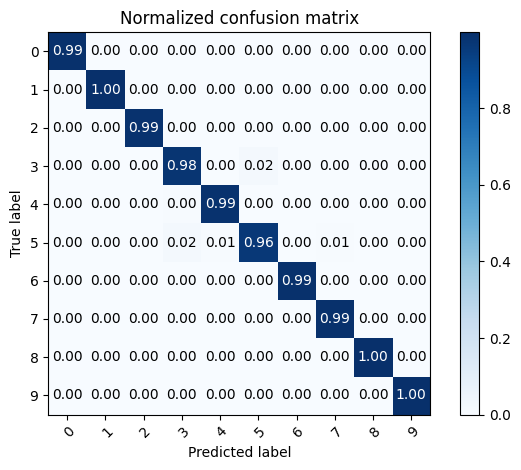
\includegraphics{figures/knn_plain_cm.png}
    \caption{Knn Dataset 1}
\end{figure}

\begin{verbatim}[Dataset 2]
\end{verbatim}

\begin{verbatim}
\end{verbatim}

\subsection{Softmax Regression}

\begin{verbatim}[Logistic Regression on Standardized Dataset 2]
\end{verbatim}

\subsection{SVM}

The last method that was tried is Support Vector Machines. This method is still
parametric and linear and practically tries to maximise a margin between
samples. 

\begin{verbatim}[Linear SVM on Dataset 1]
\end{verbatim}

Linear SVM does slightly worse than KNN with 5 neighbors, and it takes also
considerably more time to train the SVM classifier. Instead, by using a
polynomial kernel of degree 3 we obtain a slightly better performance.

\begin{verbatim}[Poly SVM Dataset 1]
\end{verbatim}

SVM with 3-degree polynomial kernel has a better performance than linear SVM and
also KNN. Although, it takes slightly more time to train it. Also, when
increasing the degree of the polynomial, performance decreases, which means the
classifier would overfit on training data.

\begin{verbatim}[Poly SVM Dataset 2]
\end{verbatim}

\subsection{Considerations}

In the end KNN and Poly SVM were the best methods on both datasets. KNN has the
advantage of taking less computational during training time, while it costs
slighly more during inference. Conversely, SVM has slighly higher accuracy but
it takes a little bit more to train it. In both cases the main problem is the
precision and recall of classes 3 and 5, which often get exchanged.

\bibliographystyle{unsrt}
\bibliography{ref}
\nocite{*}  % to include references which were not cited

\end{document}